\documentclass[11pt]{article}
\usepackage{graphicx}
\usepackage{amsmath,amsthm,amsfonts}
\usepackage{epsfig,graphics}
\usepackage{hyperref}
\usepackage{verbatim}
\usepackage{mathrsfs}
\usepackage{fancyhdr}

\setlength{\textheight}{8.5in}
\setlength{\evensidemargin}{0.0in}
\setlength{\oddsidemargin}{0.0in}
\setlength{\topmargin}{-0.5in}
\setlength{\textwidth}{6.5in}

\newtheorem{theorem}{Theorem}
\newtheorem*{theorem*}{Theorem}
\newtheorem{claim}{Claim}
\newtheorem*{claim*}{Claim}
\newtheorem{lemma}{Lemma}
\newtheorem*{lemma*}{Lemma}
\newtheorem{exercise}{Exercise}
\newtheorem*{exercise*}{Exercise}
\newtheorem{corollary}{Corollary}
\theoremstyle{definition}
\newtheorem{definition}{Definition}
\newtheorem{fact}{Fact}
\newtheorem*{fact*}{Fact}


\pagestyle{fancy}
\fancyhf{}

%\newcommand{\lecture}[5]{\handout{#1}{#2}{#3}{#4}{#5}}


% Types of Variables
\newcommand{\bvar}[1]{\mathbf{#1}} % bold variable
\newcommand{\mvar}[1]{\bvar{#1}} % matrix variable
\newcommand{\vvar}[1]{\vec{#1}} % vector variable

% Domains
\newcommand{\R}{\mathbb{R}}
\newcommand{\Z}{\mathbb{Z}}
\newcommand{\redgevec}{\R^{E}}
\newcommand{\rvertvec}{\R^{V}}
\newcommand{\rPos}{\R^{+}}
\newcommand{\rNonNeg}{\R^{\geq 0}}

% Probability Operators
\newcommand{\E}{{\mathbb{E}}}
\newcommand{\V}{{\text{Var}}}
\newcommand{\prob}{{\mathbb{P}}}

% Symbol for definitions
\newcommand{\defeq}{\stackrel{\mathrm{\scriptscriptstyle def}}{=}}

% Optimization
\DeclareMathOperator*{\argmin}{arg\,min}
\DeclareMathOperator{\Cone}{Cone}
\DeclareMathOperator{\Cut}{CUT}

% Types of Graphs
\newcommand{\nlap}{\mathscr{L}_G}
\newcommand{\pseudo}[1]{{#1}^\dagger}
\newcommand{\lapPseudo}{\pseudo{\lap}}
\newcommand{\adj}{A}
\newcommand{\incMatrix}{\mvar{B}}
\newcommand{\diag}{\operatorname{diag}}
\newcommand{\rMatrix}{\mvar{R}} % resistance matrix
\newcommand{\iMatrix}{\mvar{I}} % identity matrix
\newcommand{\Vol}{\textrm{Vol}}


% Vectors
\newcommand{\1}{\vec{1}}
\renewcommand{\dot}[1]{\langle {#1} \rangle}

%other
\DeclareMathOperator{\sgn}{sgn}


\usepackage{wrapfig}
\graphicspath{{figures/}}
\usepackage{wrapfig}

\lhead{MA 881: Homework 2}
\rhead{Benjamin Draves}

\begin{document}

\section{Exercise 1: Airways Power Diagnostics}

In this problem we are looking to evaluate the power of the airway study - a study with 4 treated and 4 untreated individuals each with 64k gene counts. Here we use DESeq2 to clean the assays matrix. Moreover, we group genes by their cell lines to adjust for correlated genes. This will greatly increase the strength of our tests to find signal in each gene. After adjusting for this affect, we run the DESeq2 analysis that gives us the resulting p-value histogram 
\begin{figure}[h!]
	\centering
	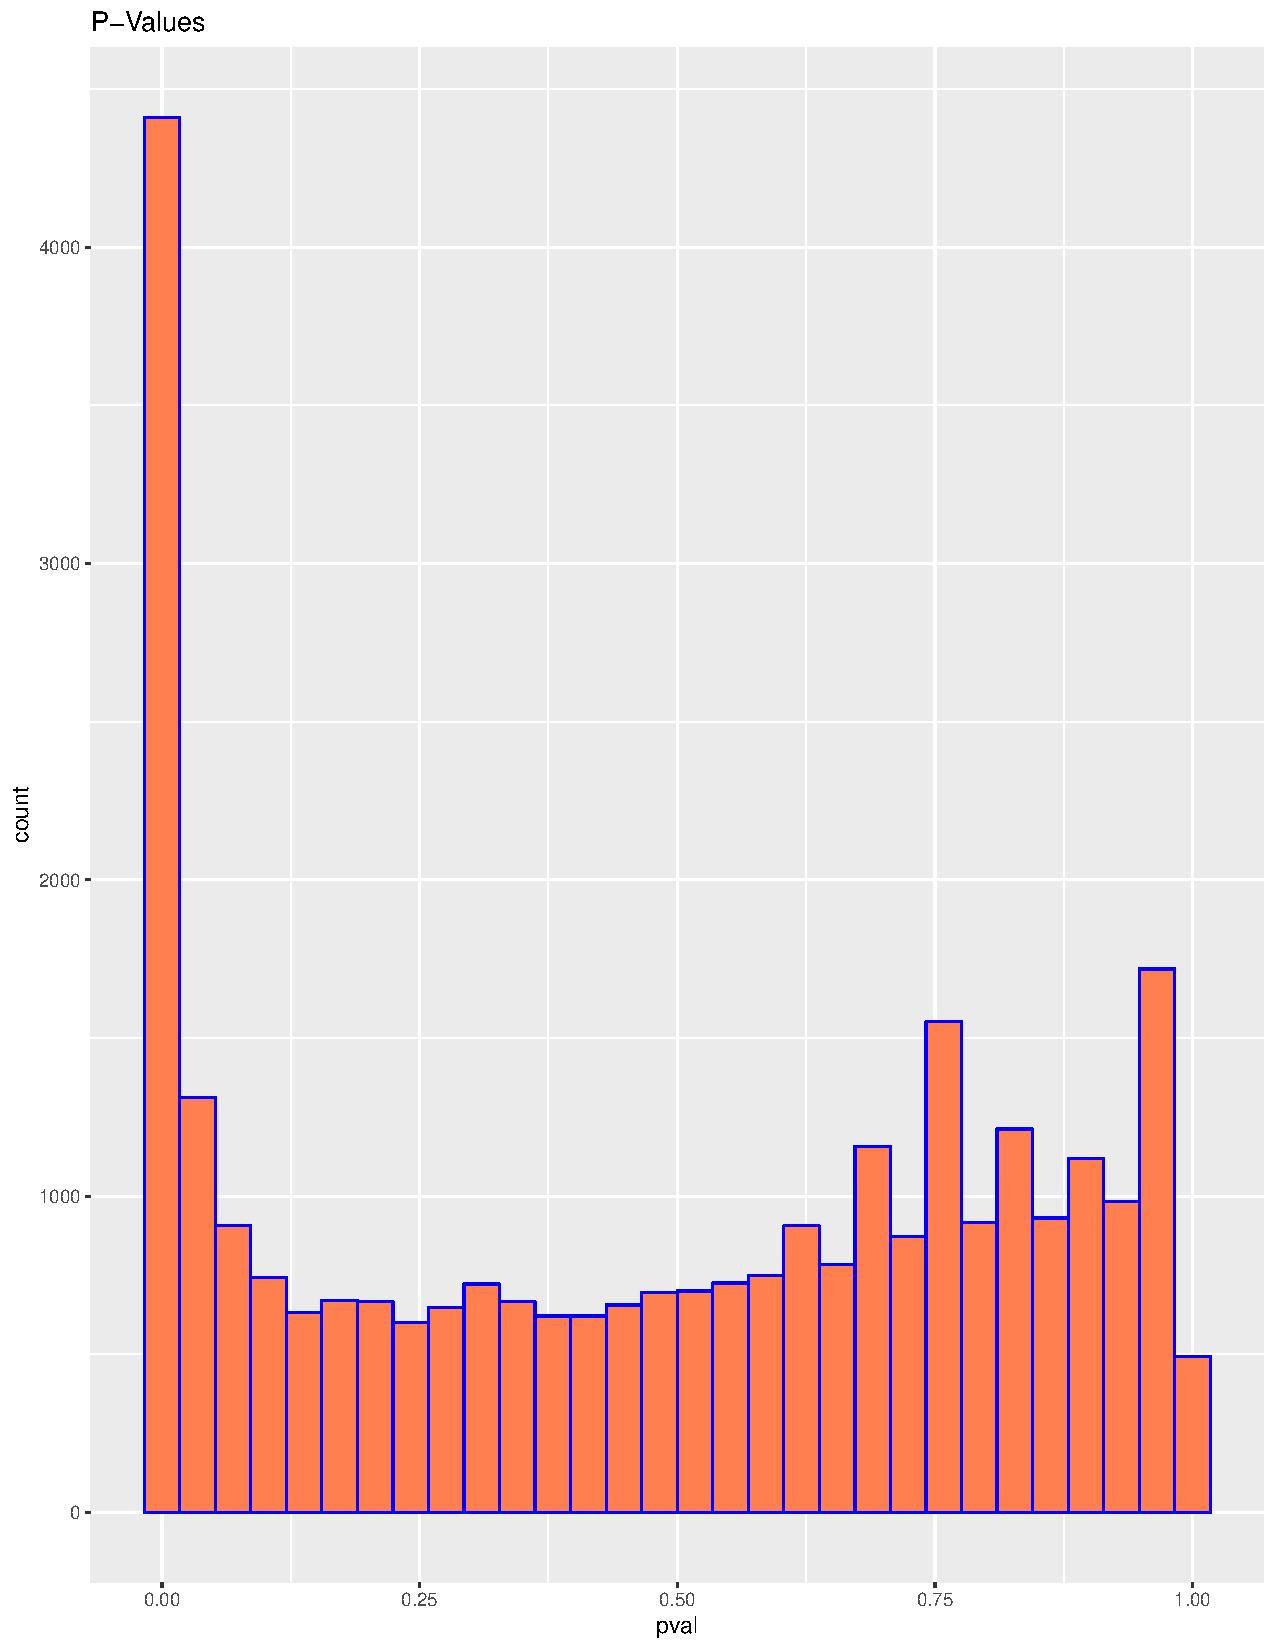
\includegraphics[scale = 0.25]{figures/p-values.pdf}
\end{figure}
Here we see that there are several genes that appear to be explaining a non-negligible amount of variance in the presence of the disease in these 8 patients. From here we can use the p-values to estimate the local false discovery rate CDF. For this, we use the Bioconductor package q-value which does just this. The results of this analysis can be found in the figure below.
\begin{figure}[h!]
	\centering
	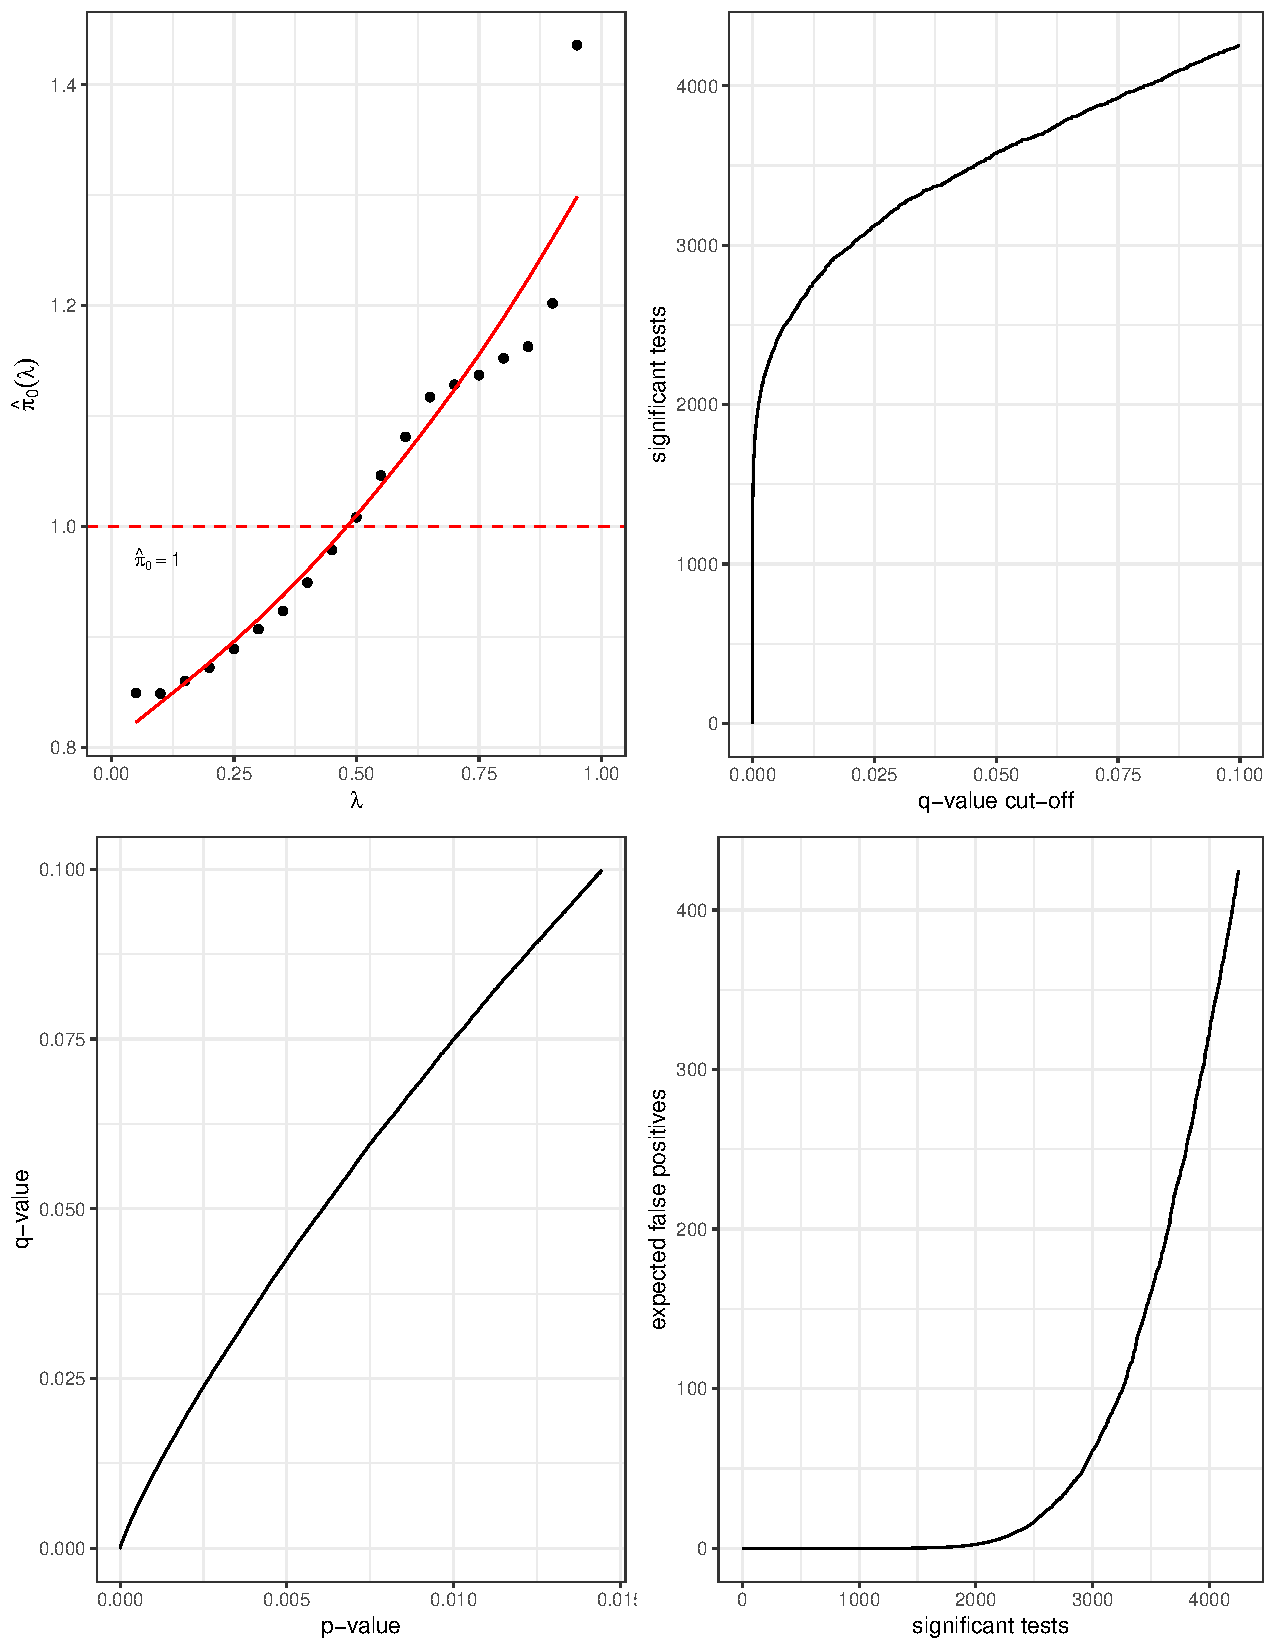
\includegraphics[scale = 0.25]{figures/q-value.pdf}
\end{figure}
The estimated local false discovery rate distribution is given in the top right panel. Here we see that this study has good power. We see that for small values of $q$ that the estimated number of significant tests is quite high. As this tolerance increases, we also see that we have a steady increase in significant tests. In either case, even when controlling for local false discovery rates, we see that several of these tests are still significant. These findings suggest that this study has good power. 



\section{Exercise 2: Book Problems}

\subsection{6.2}

\begin{wrapfigure}{R}{0.6\textwidth}
	\centering
	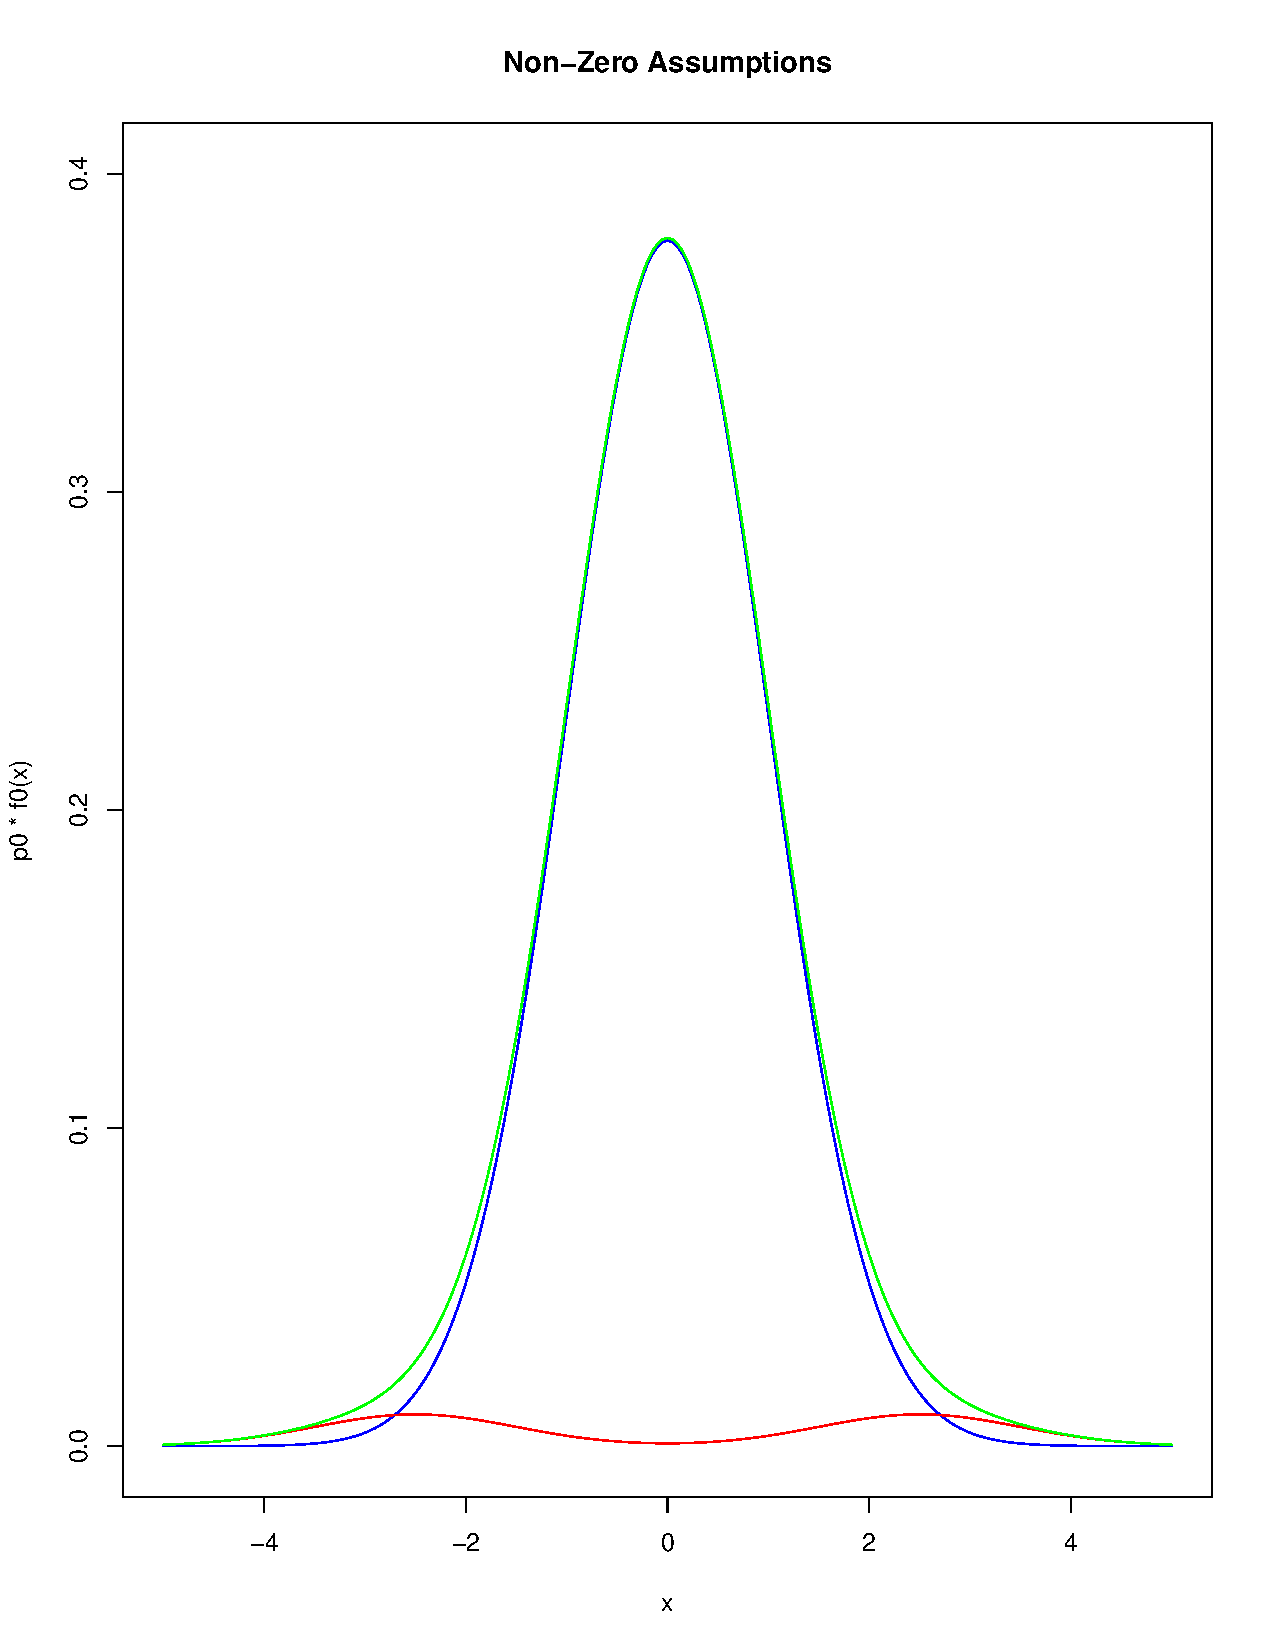
\includegraphics[scale = 0.25]{figures/non_null.pdf}
\end{wrapfigure}
Suppose that $\pi_0 = 0.95$ and $f_0\sim N(0,1)$ and the non-null distribution of $f_1 \sim \frac{1}{2}N(-2.5,1)+\frac{1}{2}N(-2.5,1)$. This then gives the three way mixture 
\begin{align*}
f(x) = \pi_0f_0(x) + (1-\pi_0)f_1(x) 
\end{align*}
Here we see that $f(x)$ is unidentifiable. For this reason we take the \textit{zero - assumption} on $\mathcal{A}_0 = [-1,1]$. Therefore, we wish to redefine the non-null and null distribution to follow this assumption. 
\begin{align*}
\widetilde{\pi}_0\widetilde{f}_0(x) &= \begin{cases}
		\pi_0f_0(x) + (1-\pi_0)f_1(x) & x\in\mathcal{A}_0\\
		\pi_0\phi_0(x) & x\not\in\mathcal{A}_0
	\end{cases}\\
	&= \begin{cases}
		\pi_0\left\{f_0(x) + \frac{1-\pi_0}{\pi_0}f_1(x)\right\}& x\in\mathcal{A}_0\\
		\pi_0\phi_0(x) & x\not\in\mathcal{A}_0
	\end{cases}
\end{align*}
Hence we see that on $\mathcal{A}_0$ the adjusted null distribution is given by the mixture $\widetilde{f}_0(x) = f_0(x) +\frac{1-\pi_0}{\pi_0}f_1(x)$ with $\widetilde{\pi}_0 = \pi_0$


\subsection{6.10}
In our case our general two sample $t$ statistic can be written as follows 
\begin{align*}
t_i &= \sqrt{n-2}\frac{(\overline{x}_A - \mu_A) - (\overline{x}_B - \mu_B)}{\sqrt{\sum_{j=1}^{n/2}(x_{ij}-\overline{x}_A)^2 +\sum_{j=n/2+1}^{n}(x_{ij}-\overline{x}_B)^2  }}
\end{align*}
Under the null distribution $\mu_A = \mu_B = 0$. Hence the above reduces to the following. 
\begin{align*}
t_i &= \sqrt{n-2}\frac{\overline{x}_A - \overline{x}_B }{\sqrt{\sum_{j=1}^{n/2}(x_{ij}-\overline{x}_A)^2 +\sum_{j=n/2+1}^{n}(x_{ij}-\overline{x}_B)^2  }}
\end{align*}
Now, notice that for each $x_{ij}$ we have that $\E(x_{ij}) = 0$ and $\V(x_{ij}) = 1 + \frac{\sigma_B^2}{4}$. If we now scale the denominator so that it has a $\chi^2$ distribution we can find the distribution of $t_i$
\begin{align*}
t_i &= \frac{\sqrt{n-2}}{\sqrt{1+\sigma^2_B/4}}\frac{\overline{x}_A - \overline{x}_B }{\sqrt{\sum_{j=n/2+1}^{n}(\frac{x_{ij}-\overline{x}_A}{\sqrt{1 + \sigma^2_B/4}})^2  +\sum_{j=n/2+1}^{n}(\frac{x_{ij}-\overline{x}_B}{\sqrt{1 + \sigma^2_B/4}})^2 }}\\
\end{align*}
Now notice here that the denominator has a $\chi^2_{n/2 - 1} + \chi^2_{n/2 - 1}  \overset{D}{=} \chi^2_{n-2}$ distribution. Hence we see that
\begin{align*}
t_i \overset{D}{=}\frac{\overline{x}_A - \overline{x}_b}{\sqrt{1+\sigma^2_B/4}}\frac{1}{\sqrt{\chi^2_{n-2}/n-2}}
\end{align*}
Moreover, as $\overline{x}_A-\overline{x}_B\sim N(0, \frac{2}{n}\left(1 + \sigma^2_B/4\right))$. With this we see that 
\begin{align*}
t_i \overset{D}{=}\sqrt{\frac{2}{n}}\frac{Z}{\sqrt{\chi_{n-2}^2}/n-2}\sim \sqrt{\frac{2}{n}}\cdot t_{n-2}
\end{align*}


To find an expression for the local false discovery rate, $fdr(t_i)$ with $\pi_0 = 1$ and $\sigma_B^2 = \frac{2}{\sqrt{n}}$ we first see that $t_i\sim \sqrt{2}\cdot t_{n-2}$. As we just argued, the new null distribution is over dispersed by a factor of $\sqrt{2}$ as compared to the normal theoretical null.  That is, under the normal theoretical null we assume that $t_i \sim t_{n-2}$. In this model we see that the variance $\V(t_i) = \frac{n-2}{n-4}\to 1$ while in reality however, this variance we know by the previous discussion is actually closer to $2$. Hence to correct for this, we see that $\frac{t_i}{\sqrt{2}}$ will have the proper large $N$ variance. Therefore, if we were to calculate this local fdr, we could approximate it as follows 

\begin{align*}
	fdr(t_i) &= \frac{\text{null}}{\text{theoretical null}} \approx \frac{\sqrt{2}f_{n-2}(t_i)}{f_{n-2}(t_i/\sqrt{2})}
\end{align*}

Lastly, we can find $\prob(fdr(t_i)\leq 0.20)$ using the previous result. 
\begin{align*}
	\prob(fdr(t_i)\leq 0.2) &= \prob\left[f_{n-2}(t_i)\leq \frac{0.2}{\sqrt{2}}f_{n-2}(t_i/\sqrt{2})\right]\\
	&=\prob\left[\left(1 + \frac{t_i^2}{18}\right)^{-19/2} \leq \frac{0.2}{\sqrt{2}}\left(1+\frac{t_i^2}{36}\right)^{-19/2}\right]\\
	&= \prob\left[t_i^2 \geq \frac{(1/5\sqrt{2})^{-2/19}1/2*36 - 18}{1 - (1/5\sqrt{2})^{-2/19}1/2}\right]
\end{align*}
Now recall that $t_i\sim t_{n-2}$. Hence $t_i^2 \sim F_{1,n-2}$. Therefore,
\begin{align*}
	\prob(fdr(t_i)\leq 0.2) = 1 - F_{1,n-2}(10.667) \approx 0.0043
\end{align*}
Therefore we see that the probability of the local false discovery being less than 0.2 is considerably low. 
\end{document}







